\section{The Chromatic Number Problem}\label{sec:chromatic}

The chromatic number problem is \emph{inherently intractable}.  Informally, this means that finding a solution for
a given input graph, regardless of the means, can take a very, very long time in the worst cases.  In fact, the
chromatic number problem is a member of a class of problems referred to as being \emph{NP-hard}, meaning that the
time to find a solution increases exponentially with the number of vertices.  Thus, trying to find an efficient but
exact method of solution that satisfies all cases is a fool's errand; about the best that can be done is to perform
better than existing well-known methods in most cases~\cite{garey}.  In order to better understand why the proposed
algorithm is inherently intractable and how to compare it with existing well-known chromatic number algorithms,
this section provides an overview of the computational complexity of algorithms.

\subsection{Problems}\label{sec:sub:problems}

The various questions asked and answered in this section can be a bit confusing, so it is essential to clearly
define the various terms that will be used.  A \emph{problem} consists of three parts:

\begin{enumerate}
\item A specific question to be answered.
\item A description of zero or more input \emph{parameters}.
\item A statement of the properties that the \emph{solution} is required to satisfy.
\end{enumerate}

An \emph{instance} of a problem is constructed by specifying particular values for each input parameter.  The
step-by-step procedure that translates the input parameters to a corresponding well-defined solution is called an
\emph{algorithm}.  To say that an algorithm \emph{solves} a problem \(\Pi\) means that the algorithm produces a
valid solution for every possible instance \(I\) of the problem \(\Pi\)~\cite{garey}.

Thus, the chromatic number problem accepts a graph \(G\) and uses an algorithm to obtain a number \(k\in\N\) where
\(k\) is the minimum value such that \(G\) is \colorable{k}.  The proposed algorithm is one such algorithm that can
be used to solve the problem.  Other examples are the Christofides (1971)~\cite{christofides} and the Corneil/Graham
(1973)~\cite{corneil} algorithms, which are compared to the proposed algorithm in later sections.

\subsection{Enigma}\label{sec:sub:enigma}

A good example of an intractable problem that involved most of the personalities who would make important
contributions to the development of a theory for computation occurred in the field of cryptography during WWII.
Although cryptography had been important in WWI, the horrors of the new era of warfare instigated by Hitler's Third
Reich brought the importance of codebreaking to the forefront.  The story of the Polish code breakers and their
\emph{bombe} device and the efforts of the British at Bletchley Park using the bombes are now legendary.  The
problem was to break the German Enigma code: given a set of ciphertext messages, convert them to intelligible
cleartext messages.  It is in the nature of this problem that the inherent intractability of some problems becomes
evident~\cite{dturing}.

The Enigma code was a letter-swapping code; however, the swap table changed with each letter.  Cleartext messages
were encoded using a typewriter-like device with the following characteristics:

\begin{enumerate}
\item Three slightly different 26-position (one for each letter) rotors that selected the swap for the current
  letter in the cleartext.  As each character was added to the ciphertext, the rotors would rotate based on their
  gear mechanisms to select the next swap, thus changing the swap table each time.
\item The ability to initialize the position of each rotor at the start of the message, which acted as a seed for the
  current cipher.
\item A plugboard where ten pairs of bidirectional manual letter swaps could be specified.
\end{enumerate}

Each of the twenty letters that made up the ten pairs on the plugboard were distinct.  Furthermore, the ordering of
the pairs was insignificant. Thus, the number of possible configurations \(N\) of the plugboard is given by:
\begin{align*}
  N &= \frac{\binom{26}{2}\binom{24}{2}\binom{22}{2}\binom{20}{2}\binom{18}{2}
  \binom{16}{2}\binom{14}{2}\binom{12}{2}\binom{10}{2}\binom{8}{2}}{10!} \\
  &=\frac{26!24!22!20!18!16!14!12!10!8!}{2^{10}24!22!20!18!16!14!12!10!8!6!10!} \\
  &=\frac{26!}{2^{10}6!10!}
\end{align*}
The German army used a set of five rotors, any three of which could be selected for a day's messages.  Thus, the
number of possible initial configurations for the army Enigma machine \(M\) was:
\[M=5\cdot4\cdot3\cdot26^3\cdot\frac{26!}{2^{10}6!10!}=158.9\times10^{18}\]
Given a ciphertext message, the bombes would (mechanically) try all possible Enigma initial configurations in an
attempt to convert the ciphertext into an intelligible cleartext message (in German).  To put this in perspective,
an Intel i7 has a speed of about \(50,000\) MIPS.  Assuming that each one of Enigma's initial configurations could
be tried in one instruction means that it would take about 100 years to try all possible combinations.  Since it
would actually take several thousand instructions to test each possible configuration, the real answer is upwards
of 100,000 years --- intractable indeed.  Furthermore, although the German army used a set of five rotors, the German
navy used a set of eight rotors.  And in 1942, both changed from a three rotor system to a four rotor system.

Clearly, a day's Enigma configuration needed to be determined within a couple hours in order to make it useful to
decode the day's messages.  It is at this point that the art of crypography comes into play.  The goal was to use
techniques like letter frequency and candidate cleartext segments to eliminate enough of the possible initial
configurations so that bombes could find the correct configuration in a reasonable amount of time.  Thus, there was
no ``aha'' moment where the Enigma code was broken once and for all.  Each new day was a new instance of the
problem that required a tremendous manual effort to eliminate possible configurations so that the bombes could try
a minimum number of combinations to arrive at the current day's solution.

\subsection{Algorithms}\label{sec:sub:algorithms}

The etymology for the word \emph{algorithm} is the Latinized name \emph{Algorithmi} for Mu\d{h}ammad ibn
M\={u}s\={a} al-Khw\={a}rizm\={\i} of algebra fame.  In Europe, the term algorithmi became synonymous with any
well-defined procedure used in mathematical problem solving, such as the division algorithm of the Babylonians,
al-Khw\={a}rizm\={\i}'s completing the square, the sieve of Eratosthenes for finding primes, and Euclid's algorithm
for find the GCD of two numbers~\cite{bernhardt}.

In today's modern computer age, the term \emph{algorithm} is used without much thought to represent a well-defined
and finite (however large) sequence of steps to solve some problem, usually within the context of a computer
program.  However, practical programmable computers didn't exist until well into the 1950s.  In fact, the formal
study of algorithms actually began in the mid to late \(19^{th}\) century as part of the effort to formalize
mathematical systems.  In order to understand why the chromatic number problem is so intractable and how to measure
that intractability, it will be helpful to investigate this fairly recent history of algorithms.

In the mid \(19^{th}\) century, the field of mathematics found itself in a bit of a crisis.  Although logic was
already the foundation of mathematics, there was a feeling that, like Euclid, many of the accepted axioms were
making too many assumptions about the involved non-defined terms, ultimately resulting in paradoxes.  One of the
most famous is the Russell paradox, communicated by British mathematician Bertrand Russell to German mathematician
Gottlob Frege circa 1902, just as Frege was about to publish a major work on the set theory foundations of
mathematical systems.  Frege had used na\"{\i}ve set theory and had made too many assumptions about the nature of
collections, an idea that was left to intuition instead of definition.  This lead to paradoxes involving sets that
were members of themselves~\cite{bernhardt}.

The first order of business was to formalize the rules for the algorithms that would be used to solve problems, and
this was done by English mathematician George Boole in 1847 and 1856 with his papers that formalized the so-called
zero-order logic, which includes: and, or, not, and implication.  This work was supplemented by the aforementioned
Frege in 1879 and independently by American mathematician Charles Peirce in 1885 when they added quantifiers to
Boole's work, resulting in the so-called first-order logic~\cite{bernhardt}.

The modern understanding of algorithms has its roots in attempts by mathematicians of the 1920s and 1930s to
formalize mathematical systems.  German mathematician David Hilbert begins in 1920 by stating what he felt were
requirements for a proper mathematical system based on some language or set of rules:

\begin{description}
\item[Completeness.] Every proposition that is true can be proven so using the rules of the system.
\item[Consistency.] No contradictions arise when following the rules.
\item[Decidability.] There exists a method for deciding whether something is true or false.
\end{description}

It is probably true that Hilbert had in mind mathematical systems based on first-order logic, which was the modus
operandi of mathematicians of the time.  However, Austrian mathematician Kurt G\"{o}del upset the apple cart in
1931 by showing that mathematical systems cannot be proved to be both complete and consistent.  Thus, only the
third requirement of decideability remained, what was commonly referred to as the
\emph{Entscheidunsproblem}~\cite{dturing}.

In 1935, British mathematician and early pioneer of programmable computing Max Newman was giving a lecture on the
Entscheidunsproblem at Cambridge.  Newman put forth of the question of whether there exists a \emph{mechanical}
process that would meet the requirements of decideability.  In the audience was a young Alan Turing who would take
the challenge for a mechical process to heart.  In 1936, Turing would submit his famous paper, ``On Computable
Numbers, with an Application to the Entscheidungsproblem~\cite{aturing},'' which provided a definition of
computable functions and a theoretical general-purpose machine to compute such functions: the A-machine, what we
know today as the Turing machine.  Turing showed that there are some problems that appear to be true; however,
there is no way to design a process to prove that they are actually true - or that the original process even
terminates with an answer (the halting problem).  Most of these types of problems involve inherent contractions
such as the Epimenides paradox: Epimenides the Cretan says that all Cretans are liars.~\cite{dturing}.  Thus,
Hilbert's third pillar was demolished.~\cite{dturing}.

It should be noted that American mathematician Alan Church arrived at the same conclusions as Turing a bit earlier
with his 1935 paper on lambda calculus.  Unlike Newton and Leibniz, Turing and Church were willing collaborators,
with Church eventually becoming Turing's PhD advisor at Princeton.  Indeed, Turing adopted the use of the lambda
calculus in his work~\cite{dturing}.

\subsection{Chromatic Number Lower Bound}\label{sec:sub:lower}

\subsection{Chromatic Number Upper Bound}\label{sec:sub:upper}

\subsection{The Christofides Algorithm}\label{sec:christofides}

\subsection{Zykov Algorithms}\label{sec:zykov}

An exhaustive, exponential-time algorithm for determining the chromatic number of a graph is derived from a
nondeterministic Turing machine technique attributed to Ukranian graph theorist Alexandre A. Zykov (1922--2013)
\cite{obit}.

\begin{figure}[h]
  \label{fig:zykov}
  \begin{center}
    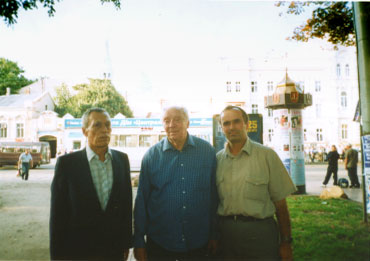
\includegraphics{zykov}
  \end{center}
  \caption{V.G Vizing (L), A.A. Zykov (C), and V.I. Voloshin (R) in Odessa (2001) \cite{voloshin}}
\end{figure}

\subsubsection{The Chromatic Polynomial}

In his 1949 paper (translated by the AMS in 1952) \cite{zykov}, Zykov addresses the question: given a graph \(G\) and
a number \(k\in\N\), how many ways are there to properly color \(G\) using at most \(k\) colors?  In fact, he is not
particularly concerned about the chromatic number, which he calls the \emph{rank}, of a graph.  To solve this problem,
Zykov notes that in any proper coloring of a graph:
\begin{enumerate}
\item Nonadjacent vertices have either the same color or different colors.
\item Adjacent vertices always have different colors.
\end{enumerate}
If nonadjacent vertices have the same color then they can be contracted and the resulting graph retains the same
\coloring{k} as the original graph.  This is demonstrated in Figure \ref{fig:zvcon}.

\begin{figure}[h]
  \label{fig:zvcon}
  \begin{center}
    \begin{minipage}{2in}
      \begin{center}
        \begin{tikzpicture}[every node/.style={labeled node}]
          \colorlet{c1}{green!25!white}
          \colorlet{c2}{blue!25!white}
          \colorlet{c3}{red!25!white}
          \node (d) [fill=c2] at (0,0) {\(d\)};
          \node (c) [fill=c3,right=of d] {\(c\)};
          \node (b) [fill=c2,above=of c] {\(b\)};
          \node (a) [fill=c1,above=of d] {\(a\)};
          \draw (a) -- (b);
          \draw (a) -- (c) -- (d) -- (a);
        \end{tikzpicture}

        \bigskip

        \(G\)
      \end{center}
    \end{minipage}
    \begin{minipage}{2in}
      \begin{center}
        \begin{tikzpicture}[every node/.style={labeled node}]
          \colorlet{c1}{green!25!white}
          \colorlet{c2}{blue!25!white}
          \colorlet{c3}{red!25!white}
          \node (bd) [fill=c2] at (0,0) {\(bd\)};
          \node (c) [fill=c3,right=of bd] {\(c\)};
          \node (a) [fill=c1,above=of bd] {\(a\)};
          \draw (a) -- (c) -- (bd) -- (a);
        \end{tikzpicture}

        \bigskip

        \(G\cdot bd\)
      \end{center}
    \end{minipage}
  \end{center}
  \caption{Same Colors with Vertex Contraction}
\end{figure}

If nonadjacent vertices have different colors then they can be joined by an edge and the resulting graph retains
the same \coloring{k} as the original graph.  This is demonstrated in Figure \ref{fig:zeadd}.

\begin{figure}[h]
  \label{fig:zeadd}
  \begin{center}
    \begin{minipage}{2in}
      \begin{center}
        \begin{tikzpicture}[every node/.style={labeled node}]
          \colorlet{c1}{green!25!white}
          \colorlet{c2}{blue!25!white}
          \colorlet{c3}{red!25!white}
          \node (d) [fill=c2] at (0,0) {\(d\)};
          \node (c) [fill=c3,right=of d] {\(c\)};
          \node (b) [fill=c2,above=of c] {\(b\)};
          \node (a) [fill=c1,above=of d] {\(a\)};
          \draw (a) -- (b);
          \draw (a) -- (c) -- (d) -- (a);
        \end{tikzpicture}

        \bigskip

        \(G\)
      \end{center}
    \end{minipage}
    \begin{minipage}{2in}
      \begin{center}
        \begin{tikzpicture}[every node/.style={labeled node}]
          \colorlet{c1}{green!25!white}
          \colorlet{c2}{blue!25!white}
          \colorlet{c3}{red!25!white}
          \node (d) [fill=c2] at (0,0) {\(d\)};
          \node (c) [fill=c3,right=of d] {\(c\)};
          \node (b) [fill=c2,above=of c] {\(b\)};
          \node (a) [fill=c1,above=of d] {\(a\)};
          \draw (a) -- (b) -- (c);
          \draw (a) -- (c) -- (d) -- (a);
        \end{tikzpicture}

        \bigskip

        \(G+bc\)
      \end{center}
    \end{minipage}
  \end{center}
  \caption{Different Colors with Edge Addition}
\end{figure}

By applying these steps recursively, all of the possible distributions of the nonadjacent nodes to independent sets
are generated.  The termination condition for each recursive path is a complete graph of some varying order \(k\).
Each node in the complete graph represents an independent set of nonadjacent nodes in the original graph that have
been combined via vertex contraction.  Thus, each complete graph of order \(k\) represents a possible \coloring{k}
of the original graph.  The complete graphs of smallest order represent chromatic colorings and their order is the
chromatic number of the original graph.

Zykov uses a graph equation syntax to record the recursive processing of a graph, where each line in the equation
represents the next recursive layer.  Isomorphic graphs are combined with a frequency multiplier at each layer.
This is demonstrated in Figure \ref{fig:greqn}.

\begin{figure}[h]
  \label{fig:greqn}
  \begin{align*}
    \begin{minipage}{0.75in}
      \begin{center}
        \begin{tikzpicture}[every node/.style={unlabeled node}]
          \node (a1) at (0,0) {};
          \node (a2) [right=of a1] {};
          \node (a3) [above=of a2] {};
          \node (a4) [above=of a1] {};
          \draw (a3) -- (a4) -- (a1) -- (a2) -- (a4);
        \end{tikzpicture}
      \end{center}
    \end{minipage} &=
    \begin{minipage}{0.75in}
      \begin{center} 
        \begin{tikzpicture}[every node/.style={unlabeled node}]
          \node (b1) at (0,0) {};
          \node (b2) [above=of b1] {};
          \node (b3) [right=of b1] {};
          \draw (b1) -- (b2) -- (b3) -- (b1);
        \end{tikzpicture}
      \end{center}
    \end{minipage} +
    \begin{minipage}{0.75in}
      \begin{center}
        \begin{tikzpicture}[every node/.style={unlabeled node}]
          \node (c1) at (0,0) {};
          \node (c2) [right=of a1] {};
          \node (c3) [above=of a2] {};
          \node (c4) [above=of a1] {};
          \draw (c2) -- (c3) -- (c4) -- (c1) -- (c2) -- (c4);
        \end{tikzpicture}
      \end{center}
    \end{minipage} \\
    &= \begin{minipage}{0.75in}
      \begin{center} 
        \begin{tikzpicture}[every node/.style={unlabeled node}]
          \node (b1) at (0,0) {};
          \node (b2) [above=of b1] {};
          \node (b3) [right=of b1] {};
          \draw (b1) -- (b2) -- (b3) -- (b1);
        \end{tikzpicture}
      \end{center}
    \end{minipage} +
    \begin{minipage}{0.75in}
      \begin{center} 
        \begin{tikzpicture}[every node/.style={unlabeled node}]
          \node (b1) at (0,0) {};
          \node (b2) [above=of b1] {};
          \node (b3) [right=of b1] {};
          \draw (b1) -- (b2) -- (b3) -- (b1);
        \end{tikzpicture}
      \end{center}
    \end{minipage} +
    \begin{minipage}{0.75in}
      \begin{center}
        \begin{tikzpicture}[every node/.style={unlabeled node}]
          \node (c1) at (0,0) {};
          \node (c2) [right=of a1] {};
          \node (c3) [above=of a2] {};
          \node (c4) [above=of a1] {};
          \draw (c2) -- (c3) -- (c4) -- (c1) -- (c2) -- (c4);
          \draw (c1) -- (c3);
        \end{tikzpicture}
      \end{center}
    \end{minipage} \\
    &= 2
    \begin{minipage}{0.75in}
      \begin{center} 
        \begin{tikzpicture}[every node/.style={unlabeled node}]
          \node (b1) at (0,0) {};
          \node (b2) [above=of b1] {};
          \node (b3) [right=of b1] {};
          \draw (b1) -- (b2) -- (b3) -- (b1);
        \end{tikzpicture}
      \end{center}
    \end{minipage} +
    \begin{minipage}{0.75in}
      \begin{center}
        \begin{tikzpicture}[every node/.style={unlabeled node}]
          \node (c1) at (0,0) {};
          \node (c2) [right=of a1] {};
          \node (c3) [above=of a2] {};
          \node (c4) [above=of a1] {};
          \draw (c2) -- (c3) -- (c4) -- (c1) -- (c2) -- (c4);
          \draw (c1) -- (c3);
        \end{tikzpicture}
      \end{center}
    \end{minipage} \\
    &= 2K_3+K_4
  \end{align*}
  \caption{Zykov Graph Equation}
\end{figure}

Determining whether two graphs are isomorphic is hard, so combining isomorphic graphs in all but the very simple
cases should be skipped; the complete graphs resulting from the further processing of two isomorphic graphs will
eventually be combined anyway by the end.

Zykov was trying to determine the number of \coloring{k}s of a graph without color indifference: each permutation
of colors for a particular distribution is considered unique.  Thus, Zykov multiplied each complete graph
coefficient in the final line of a graph equation by the number of permutations from selecting the order \(n\) of
the particular complete graph from \(k\) colors:
\[k^{(n)}=k(k-1)(k-2)\cdots(k-n+1)\]
Thus, the total number of unique colorings from the example shown in Figure \ref{fig:greqn} using \(k\) colors
would be:
\[M(G,k)=2k^{(3)}+k^{(4)}\]
This is known as the factorial form of the \emph{chromatic polynomial} for the graph.  The corresponding
\emph{expanded form} is:
\[M(G,k)=k^4-4k^3+5k^2-2k\]
Read (1968) \cite{read} expands on the construction of the factorial form of the chromatic polynomial for a graph
and proves several theorems regarding the expanded form.  Some examples are:
\begin{enumerate}
\item \(M(G,k)=M(G\cdot uv)+M(G+uv)\), where \(u\) and \(v\) are any two nonadjacent vertices in the current
  recursive step.
\item The degree of M(G,k) is the order of \(G\).
\item The highest order coefficient is \(1\).
\item There is no constant term.
\item The terms alternate in sign.
\end{enumerate}
In fact, Read shows that the expanded form is actually an inclusion-exclusion equation resulting from starting with
all possible proper and improper colorings \(k^n\) and then subtracting the improper colorings.

\subsubsection{An Exhaustive Algorithm}

Corneil and Graham extend Zykov's work with the following theorem \cite{corneil}:

\begin{theorem}[Corneil and Graham, 1973]
  \label{thm:corneil}
  Let \(G\) be a graph and let \(u\) and \(v\) be two nonadjacent vertices in \(G\):
  \[\X(G)=\min\set{\X(G\cdot uv),\X(G+uv)}\]
\end{theorem}

Zykov's method combined with Theorem \ref{thm:corneil} can be used to construct an exhaustive algorithm for finding
the chromatic number and a chromatic coloring for a graph \(G\).  We define \(S\) to be a first-in-first out (FIFO)
stack of graphs and \(X\) to be the last found complete graph of the smallest order.  Each vertex in \(X\)
represents a set of contracted vertices.
\begin{enumerate}
\item Construct a graph \(G'\) that is isomorphic to \(G\) and where each vertex in \(G'\) is a list of contracted
  vertices initialized to a one element list containing the corresponding vertex in \(G\).
\item Push \(G'\) onto \(S\).
\item \label{step:zempty} If \(S\) is empty then return \(n(X)\) and \(X\).
\item \label{step:zcheck} If the graph on the top of \(S\) is complete:
  \begin{enumerate}
  \item Pop the graph off of the top of \(S\) and save it as \(H\).
  \item If \(X\) is not set or \(n(H)<n(X)\) then let \(X=H\).  Otherwise, discard \(H\).
  \item Go to step \ref{step:zempty}.
  \end{enumerate}
\item The graph on the top of \(S\) is not complete.  Pop the graph off of \(S\) and save it as \(H\).
\item Pick any two nonadjacent vertices \(u\) and \(v\) in \(H\).
\item Push \(H+uv\) onto \(S\).
\item Construct \(H'=H\cdot uv\), where the contracted vertex list for the new contracted vertex is a concatenation
  of the lists for \(u\) and \(v\).
\item Push \(H'\) onto \(S\).
\item Go to step \ref{step:zcheck}.
\end{enumerate}

The steps of this algorithm can be tracked via a so-called \emph{Zykov tree} \cite{corneil}.  The Zykov tree for
the example in Figure \ref{fig:greqn} is shown in Figure \ref{fig:ztree}.  Note that the exhaustive algorithm
corresponds to a depth-first walk of the tree.

\begin{figure}[h]
  \label{fig:ztree}
  \begin{center}
    \begin{tikzpicture}
      \node (a) [draw,circle] at (0,0) {
        \begin{tikzpicture}[every node/.style={unlabeled node}]
          \node (a1) at (0,0) {};
          \node (a2) [right=of a1] {};
          \node (a3) [above=of a2] {};
          \node (a4) [above=of a1] {};
          \draw (a3) -- (a4) -- (a1) -- (a2) -- (a4);
        \end{tikzpicture}
      };
      \node (b) [draw,circle,below left=of a] {
        \begin{tikzpicture}[every node/.style={unlabeled node}]
          \node (b1) at (0,0) {};
          \node (b2) [above=of b1] {};
          \node (b3) [right=of b1] {};
          \draw (b1) -- (b2) -- (b3) -- (b1);
        \end{tikzpicture}
      };
      \node (c) [draw,circle,below right=of a] {
        \begin{tikzpicture}[every node/.style={unlabeled node}]
          \node (c1) at (0,0) {};
          \node (c2) [right=of a1] {};
          \node (c3) [above=of a2] {};
          \node (c4) [above=of a1] {};
          \draw (c2) -- (c3) -- (c4) -- (c1) -- (c2) -- (c4);
        \end{tikzpicture}
      };
      \node (d) [draw,circle,below left=of c] {
        \begin{tikzpicture}[every node/.style={unlabeled node}]
          \node (d1) at (0,0) {};
          \node (d2) [above=of d1] {};
          \node (d3) [right=of d1] {};
          \draw (d1) -- (d2) -- (d3) -- (d1);
        \end{tikzpicture}
      };
      \node (e) [draw,circle,below right=of c] {
        \begin{tikzpicture}[every node/.style={unlabeled node}]
          \node (c1) at (0,0) {};
          \node (c2) [right=of a1] {};
          \node (c3) [above=of a2] {};
          \node (c4) [above=of a1] {};
          \draw (c2) -- (c3) -- (c4) -- (c1) -- (c2) -- (c4);
          \draw (c1) -- (c3);
        \end{tikzpicture}
      };
      \draw (a) edge (b) edge (c);
      \draw (c) edge (d) edge (e);
    \end{tikzpicture}
  \end{center}
  \caption{A Zykov Tree}
\end{figure}

\subsubsection{Branch and Bound Strategies}

Using a Zykov tree suggests that the exhaustive algorithm is a candidate for a branch-and-bound solution, where the
branching is accomplished via vertex contraction and edge addition and the bounding is some method to prematurely
terminate a branch.  Corneil and Graham suggest such a bounding technique through the determination of so-called
\(\a\)-clusters; however, the algorithm for finding such clusters has \(\BO(n^3)\) runtime complexity.
